\begin{Problem}
	Wir ändern die Gruppendefinition aus Definition 2.3 ab, indem wir für eine Menge $G$ mit einer zweistelligen Verknüpfung $\cdot$ und einem Element $e\in G$ fordern:
	\begin{parts}
		\item Es gilt $(a\cdot b)\cdot c=a\cdot(b\cdot c)$ für alle $a,b,c\in G$.	
		\item Es gilt $a\cdot e=a$ für alle $a\in G$.
 \item[\refstepcounter{enumi}(\alph{enumi}\textquotesingle)] Zu jedem $a \in G$ gibt es ein Element $b\in G$ mit $b\cdot a = e$
	\end{parts}
Ist dann $G$ stets eine Gruppe?
\end{Problem}
\begin{proof}
	Nein. Sei $x\cdot y=x$. Es ist assoziativ, weil $x\cdot (y \cdot z)=x=(x\cdot y)\cdot z$. Es gilt auch $x\cdot e=x~\forall x$. Außerdem gilt $e\cdot x=e~\forall x\in G$. 
	Aber es gilt f\"{u}r alle $e\neq x\in G$, dass $x\cdot y=x\neq e~\forall y \in G$. $G$ ist dann keine Gruppe.
\end{proof}

\begin{Problem}
		Sei $n\in N$ mit $n\ge 3$ fixiert. Wir setzen $\alpha := \exp ( 2\pi i / n ) \in \C$ und definieren die folgenden zwei Abbildungen:
	\[
		s:\C\to \C, \qquad z\to \overline{z}\qquad\text{sowie}\qquad r:\C\to\C, z\to\alpha z
	.\] 
	Das neutrale Element der Gruppe $\text{Sym}(\C)$ bezeichnen wir mit $e$ und mit $\cdot$ die Verkettung von Funktionen.
	\begin{parts}
	\item Zeigen Sie, dass $s^2=e$ und $r\cdot s\cdot r=s$ gelten.
	\item Zeigen Sie, dass für $k\in\N$ genau dann $r^k = e$ gilt, wenn $n|k$ ist.
	\item Zeigen Sie, dass $r$ und $s$ Elemente der symmetrischen Gruppe $\text{Sym}(\C)$ sind.
	\item Zeigen Sie, dass $s\cdot r^k = r^{-k} \cdot s$ für alle $k \in\N$ gilt.
	\item Zeigen Sie, dass zu jedem $k\in \N$ ein $t\in \N$ mit $r^{-k}=r^t$ existiert.
	\item Beschreiben Sie das Abbildungsverhalten von $r$ und $s$ geometrisch.
	\item Folgern Sie aus (a)–(e), dass $\{r^x \cdot s^y | x, y \in \Z\} = \{r^a \cdot s^b | 0 \le a < n\text{ und }0 \le b < 2\}$ gilt.
	\item Zeigen Sie, dass $D_n := \{r^a \cdot s^b |0 \le a < n\text{ und }0 \le b < 2\}$ eine Gruppe ist.
	\item Beweisen Sie, dass $|D_n| = 2n$ gilt.
	\item Zeigen Sie, dass $D_n$ nicht abelsch ist.
	\end{parts}
\end{Problem}
\begin{proof}
\begin{parts}
\item  $s^2=e$ folgt aus $\overline{\overline{z}}=z$. Es gilt
\begin{align*}
	(r\cdot s\cdot r)(z)=&(r\cdot s)\left( \exp(2\pi i / n)z \right) \\
	=& r\left( \exp(-2\pi i / n)\overline{z} \right) \\
	=& \exp(2\pi i / n)\exp(-2\pi i / n )\overline{z}\\
	=& \overline{z}
\end{align*}
Also $r\cdot s\cdot r = s$.
\item Wir wissen,  $r^k(z)=\exp(2\pi i k / n)z$. $r^k=e$ genau dann, wen $\exp(2\pi i k / n)=1$, also $n | k$.
\item Sie sind bijektiv. Wir schreiben einfach die Umkehrfunktion. 
	\begin{equation}\tag{a}
		s^{-1}=s
	\end{equation}
	\begin{align*}
		f(x)=&\exp(-2\pi i / n)x\\
		r\circ f=&e=f\circ r
	\end{align*}
\item 
	 \begin{align*}
		 (s\cdot r^k)(z)=& s\left( \exp\left( 2\pi i k / n \right) z \right) \\
		 =& \exp\left( -2\pi i k / n \right) \overline{z}\\
		 (r^{-k}\cdot s)(z)=&\left( r^{-k} \right) (\overline{z})\\
		 =& \exp(-2\pi i k / n)\overline{z}\\
		 =&(s\cdot r^k)(z)
	\end{align*}
\item Sei $t=-k+pn, p\in \N$, f\"{u}r $p$ hinreichend groß, damit $t>0$ und daher $p\in \N$. Es gilt
	 \[
		 s^t=s^{-k+pn}=s^{-k}s^{pn}=s^{-k}(s^n)^p=s^{-k}
	.\] 
\item\noindent\\ 
	\begin{center}
		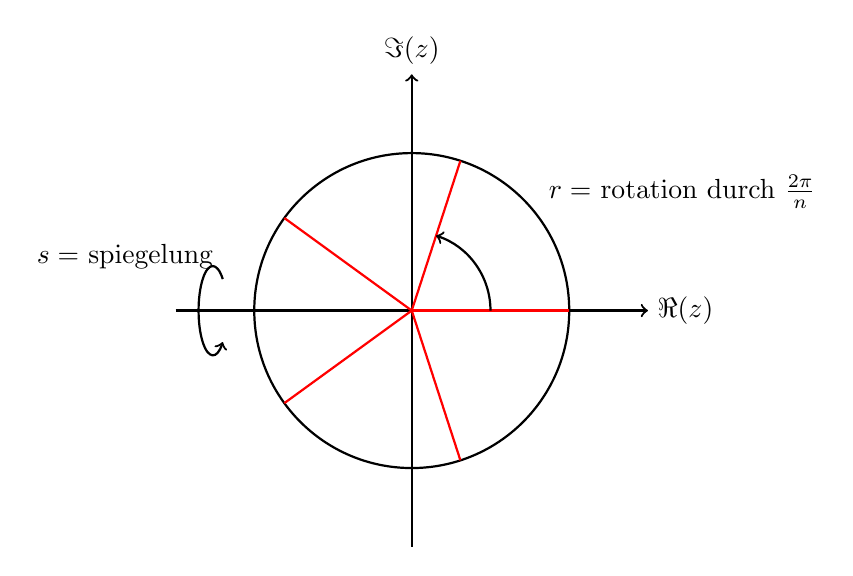
\begin{tikzpicture}[scale=2]
			\draw[thick, ->] (-1.5,0) -- (1.5,0);
			\draw[thick, ->] (0,-1.5) -- (0,1.5);
			\draw[thick] (0,0) circle (1);
			\foreach \x in {0,1,2,3,4}
			{
				\draw[thick,red] (0,0) -- ({cos(360*\x/5)},{sin(360*\x/5)});
			}
			\draw[thick, ->] (0.5,0) arc(0:72:0.5);
			\draw ({cos(36)},{sin(36)}) node[anchor=south west] {$r=$ rotation durch $\frac{2\pi}{n}$}; 
			\draw[thick,->] (-1.2,0.2) arc (45:315:0.09 and {0.2*sqrt(2)});
			\draw (-1.2,0.2) node[anchor=south east]{$s=$ spiegelung};
			\draw (1.5,0) node[anchor=west] {$\Re(z)$};
			\draw (0,1.5) node[anchor=south] {$\Im(z)$};
		\end{tikzpicture}
	\end{center}
\item Sei $y=2n+b, b\in \N$. Dann ist 
	\[
		s^y=s^{2n+b}=s^{2n}\cdot s^b=e\cdot s^b=s^b
	.\] 
\item 
	\begin{enumerate}[label=(\roman*)]
		\item $D_n$ ist abgeschlossen
			\begin{align*}
				r^a\cdot s^b\cdot r^{a'}\cdot s^{b'}=&r^a\cdot r^{-a'}\cdot s^b\cdot s^{b'} & \text{(d)}\\
				=&r^{a-a'}s^{b+b'}\\
				\in& D_n & \text{(g)}
			\end{align*}
		\item $D_n$ ist assoziativ wegen der Assoziatitivät von Funktionverkettung.
		\item Neutrales Element

			$a=0,b=0,r^0\cdot s^0=e\in D_n$.
		\item Inverses Element
		 \[
			 s^{-b}\cdot r^{-a}\cdot r^a\cdot s^b=s^{-b}\cdot(r^{-a}\cdot r^a)\cdot s^b=s^{-b}\cdot s^b=e
		.\] 
		Außerdem gilt
		\begin{align*}
			s^{-b}\cdot r^{-a}=&r^a\cdot s^{-b} &\text{(d)}\\
			=&r^a\cdot s^c,~0\le c < 2 & \text{(a)}
		\end{align*}
	\end{enumerate}
\item Es gibt genau $n$ Möglichkeiten für $a$, und $2$ Möglichkeiten f\"{u}r $b$. Daraus folgt $|D_n|=2n$.
\item Wir haben $s\cdot r^k=r^{-k}\cdot s$ (d), und müssen nur $k$ finden, sodass $r^k\neq r^{-k}$. $k=1$ ist ein Gegenbeispiel.\qedhere
\end{parts}
\end{proof}
